\documentclass[10pt,b5paper,titlepage]{book}

\usepackage[utf8]{inputenc}
\usepackage{amsmath}
\usepackage{amsfonts}
\usepackage{amssymb}
%\usepackage{xcolor}
\usepackage{color}
\usepackage{graphicx}

% python - needs pip install Pygments
\usepackage{minted}
\usemintedstyle{native}

\usepackage{hyperref}

\author{Jan Tomek}
\title{\bf FEM Practices}

% python code format
\setminted[python]{breaklines, framesep=2mm, fontsize=\footnotesize, numbersep=5pt}
\newminted[python]{python}{linenos=true,
                           frame=lines,
                           baselinestretch=1.2,
                           mathescape,
                           xleftmargin=1cm,
                           framesep=2mm,
                           fontsize=\footnotesize}

\setlength{\parindent}{0ex}
\setlength{\parskip}{1em plus 0.1em minus 0.2em}
\renewcommand{\labelitemi}{$\bullet$}
\renewcommand{\labelitemii}{$\bullet$}
\renewcommand{\labelitemiii}{$\bullet$}
\renewcommand{\labelitemiv}{$\bullet$}

%Commands definitions
\newcommand\setbackgroundcolour{\pagecolor[rgb]{0.15,0.15,0.15}}
\newcommand\settextcolour{\color[rgb]{0.9,0.9,0.9}}
\newcommand\invertbackgroundtext{\setbackgroundcolour\settextcolour}

% equal by definition
\newcommand*\eqd{\stackrel{\triangle}{=}}

% {name}[number of arguments][1st default value] etc..
% the argument value is then inserted at #argument_number
\newenvironment{bbox}[1][1.0]
{
    \begin{center}
        \begin{tabular}{|p{#1\textwidth}|}
            \hline\\
}
{
            \\\\\hline
        \end{tabular}
    \end{center}
}

\newenvironment{bboxtitle}[1][1.0]
{
    \begin{center}
        #1\\[1ex]
        \begin{tabular}{|p{#1\textwidth}|}
            \hline\\
}
{
            \\\\\hline
        \end{tabular}
    \end{center}
}

\newenvironment{ematrix}
{
    \begin{eqnarray}
        \begin{aligned}
}
{
        \end{aligned}
    \end{eqnarray}
}

%Command execution.
%If this line is commented, then the appearance remains as usual.
\invertbackgroundtext

\begin{document}

\maketitle

\tableofcontents

\chapter{Dynamics}

\section{SDOF system}

\subsection{Definition}

Let:

\begin{equation}
    m \ddot{u}(t) + c \dot{u}(t) + k u(t) = f(t)
\end{equation}

or:

\begin{equation}
    m a(t) + c v(t) + k u(t) = f(t)
\end{equation}

be the \textbf{SDOF equation of motion}, then the following applies:

\begin{ematrix}
    \omega^2 &= \frac{k}{m} \\
    \omega &= \sqrt{\frac{k}{m}} \\
    f &= \frac{\omega}{2 \pi} \\
    T &= \frac{1}{f}
\end{ematrix}

where:\\
$ \omega $ is radial eigenfrequency [rad/s],\\
$ f $ is eigenfrequency [Hz] and\\
$ T $ is period [s]

The simplest vibratory syslem can be described by a single mass connected to a spring
(and possibly a dashpot). The mass is allowed to travel only along the spring elongation
direction. Such systems are called \textit{Single Degree-of-Freedom} (\textbf{SDOF})
systems and are shown in the figure.

\begin{figure}[ht]
    \centering
    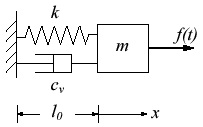
\includegraphics[width=0.90\textwidth]{img/SDOF_plot.png}
    \caption{SDOF system with a linear spring and dashpot}
    \label{fig:SDOF-plot-png}
\end{figure}

\subsection{Equation of Motion for SDOF Systems}

SDOF vibration can be analyzed by \textbf{Newton's second law of motion},
$ F = m a $. The analysis can be easily visualised with the aid of a
\textbf{free body diagram},

\begin{figure}[ht]
    \centering
    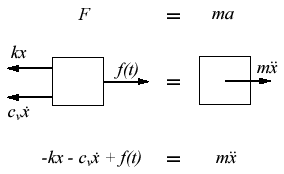
\includegraphics[width=0.90\textwidth]{img/SDOF_FreeBodyDiagram.png}
    \caption{SDOF Free Body Diagram}
    \label{fig:SDOF-freebodydiagram-png}
\end{figure}

The resulting equation of motion is a
\textbf{second order, non-homegeneous, ordinary differential equation}:

\begin{equation}
    m \ddot{u} + c \dot{u} + k u = f(t)
        \left\{ \begin{matrix}
                u(t=0) = u_0\\
                \dot{u}(t=0) = \dot{u}_0
          \end{matrix} \right.
\end{equation}

with the initial conditions $ u_0 $ and $ \dot{u}_0 $.


\subsection{Time Solution for Undamped SDOF Systems}

\textit{https://www.efunda.com/formulae/vibrations/sdof\_free\_undamped.cfm}

The equation of motion derived in the definition can be simplified to:

\begin{equation}
    m \ddot{u} + k u = f(t)
        \left\{ \begin{matrix}
                u(t=0) = u_0\\
                \dot{u}(t=0) = \dot{u}_0
          \end{matrix} \right.
\end{equation}

This equation of motion is a
\textbf{second order, homegeneous, ordinary differential equation} (ODE). If the mass
and spring stiffness are constants, the ODE becomes a
\textbf{linear, homogeneous ODE with constant coefficients} and can be solved
by the Characteristic Equation method. The characteristic equation for this
problem is:

\begin{equation}
    m s^2 + k = 0
\end{equation}

which determines the 2 independent roots for the undamped vibration problem.
The final solution (that contains the 2 independent roots from the characteristic
equation and satisfies the initial conditions) is:

\begin{ematrix}
    u(t) &= c_1 e^{i \omega_n t} + c_2 e^{- \omega_n t}\\
         &= d_1 \cos{\omega_n t} + d_2 \sin{\omega_n t} \\
    \implies u(t) &= u_0 \cos{\omega_n t} + \frac{\dot{u}_0}{\omega_n} \sin{\omega_n t}
\end{ematrix}

The natural frequency $ \omega_n $ is defined by:

\begin{equation}
    \omega_n = \sqrt{\frac{k}{m}}
\end{equation}

and depends only on the system mass and the spring stiffness (i.e. any damping will
not change the natural frequency of a system).

Alternatively, the solution may be expressed by the equivalent form,

\begin{equation}
    u(t) = A_0 \cos{\omega_n t - \phi_0}
\end{equation}

where the amplitude $ A_0 $ and the intial phase $ \phi_0 $ are given by:

\begin{ematrix}
    A_0 &= \sqrt{u_0^2 + \left(\frac{\dot{u}_0}{\omega_n}\right)^2}\\
    \phi_0 &= \tan^{-1}\frac{\dot{u}_0}{u_0 \omega_n}
\end{ematrix}

\begin{figure}[ht]
    \centering
    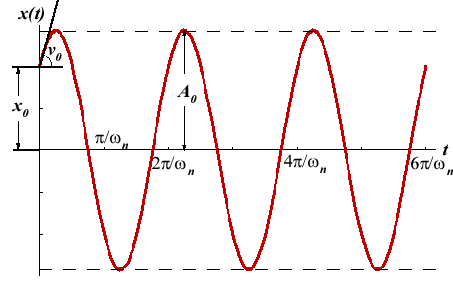
\includegraphics[width=0.90\textwidth]{img/SDOF_Undamped_Response.png}
    \caption{SDOF Undamped sample time behavior}
    \label{fig:SDOF-undamped-response-png}
\end{figure}

Note that an assumption of zero damping is typically not accurate. In reality,
there almost always exists some resistance in vibratory systems. This reistance
will damp the vibration and dissipate energy, the oscillatory motion caused by the
initial disturbance will eventually be reduced to zero.







\section{Damping}

\subsection{Rayleigh Damping}
\textit{https://www.simscale.com/knowledge-base/rayleigh-damping-coefficients/}

Let \textbf{Rayleigh Damping} be defined as:

\begin{equation}
    c = \alpha k + \beta m
\end{equation}

where:\\
$ c $ is damping value [-],\\
$ \alpha $ is stiffness dependent damping coefficient,\\
$ \beta $ is inertia (mass) dependent damping coefficient,\\
$ m $ is mass and\\
$ k $ is stiffness.

Thus, substituting this relation to the equation of motion:

\begin{ematrix}
    m \ddot(u) + \left(\alpha k + \beta m \right) \dot{u} + k u &= f(t) & \space \vert \times \frac{1}{m}\\
    \ddot{u} + \left(\alpha \frac{k}{m} + \beta \frac{m}{m} \right) \dot{u} + \frac{k}{m} u
    &= \frac{f(t)}{m} & \space \vert \frac{k}{m} = \omega_n^2 \\
    \ddot{u} + \left(\alpha \omega_n^2 + \beta \right) \dot{u} + \omega_n^2 u &= \frac{f(t)}{m} & \space
\end{ematrix}

Damping Ratio:

\begin{ematrix}
    \zeta &= \frac{c}{2 m \omega_n}\\
    \zeta &= \frac{1}{2 m \omega_n} \left( \alpha k + \beta m \right)\\
    \zeta &= \frac{1}{2} \left( \alpha \omega_n + \frac{\beta}{\omega_n} \right)
\end{ematrix}

where:\\
$ \zeta $ is damping ratio,\\
$ c $ is damping value [-],\\
$ m $ is mass and\\
$ \omega_n $ is natural frequency [rad/s]

Substituting back:

\begin{equation}
    \ddot{u} + 2 \zeta \omega_n \dot{u} + \omega_n^2 k u = \frac{f(t)}{m}
\end{equation}


When \textbf{Damping is proportional to inertia}:

In this case, the stiffness coefficient $ \alpha = 0 $ and thus:

\begin{equation}
    \zeta = \frac{\beta}{2 \omega_n}
\end{equation}

For a given constant value of $ \beta $, it is seen that the damping is inversely
proportional to the natural frequency, as shown in the illustration:

\begin{figure}[ht]
    \centering
    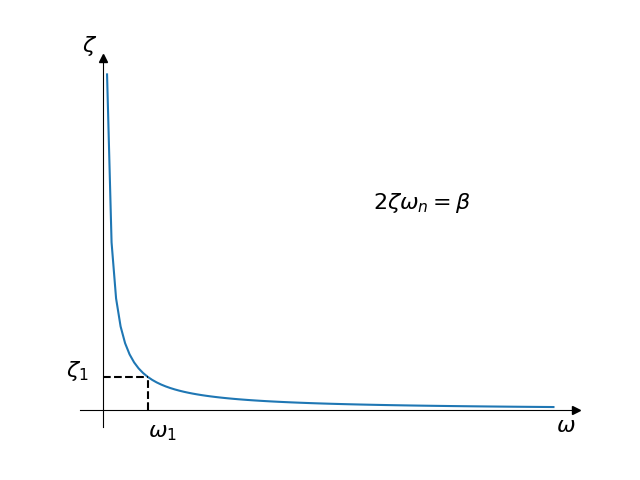
\includegraphics[width=0.90\textwidth]{img/inertia_dependent_damping.png}
    \caption{Schematic of damping proportional to inertia}
    \label{fig:inertia-dependent-damping-png}
\end{figure}

Moreover, if one computes $ \beta $ from the damping ration $ \zeta_1 $ at a given
natural frequency $ \omega_1 $, all the natural frequencies below it will be amplified
and the frequencies above it will be attenuated. The effect is more dramatic the farther
the frequencies are from the reference value.

When \textbf{Damping is proportional to stiffness}:

In this case, the mass coefficient $ \beta = 0 $ and thus:

\begin{equation}
    \zeta = \frac{1}{2} \alpha \omega_n
\end{equation}

It is seen that, contrary to the first case, here the damping id directly proportional
to the natural frequency:

\begin{figure}[ht]
    \centering
    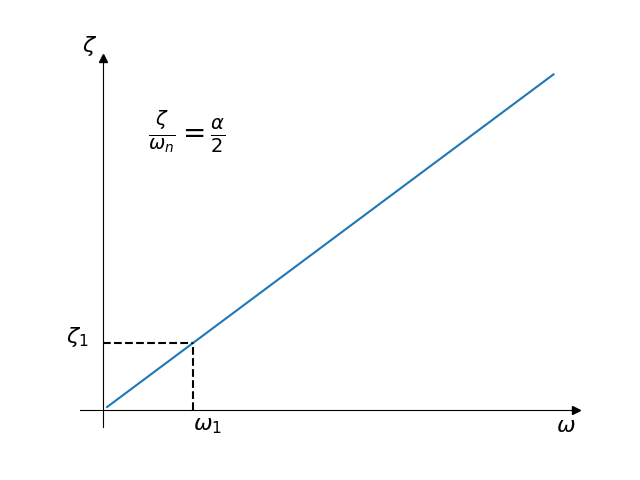
\includegraphics[width=0.90\textwidth]{img/stiffness_dependent_damping.png}
    \caption{Schematic of damping proportional to stiffness}
    \label{fig:stiffness-dependent-damping-png}
\end{figure}

If one computes $ \alpha $ from the damping ratio $ \zeta_1 $ at a natural
frequency $ \omega_1 $, then the natural frequencies below will be attenuated and
the frequencies above will be amplified.

\textbf{General Case}:

In the case of using the model with two parameters, the proportionality of damping
against frequency is convex:

\begin{figure}[ht]
    \centering
    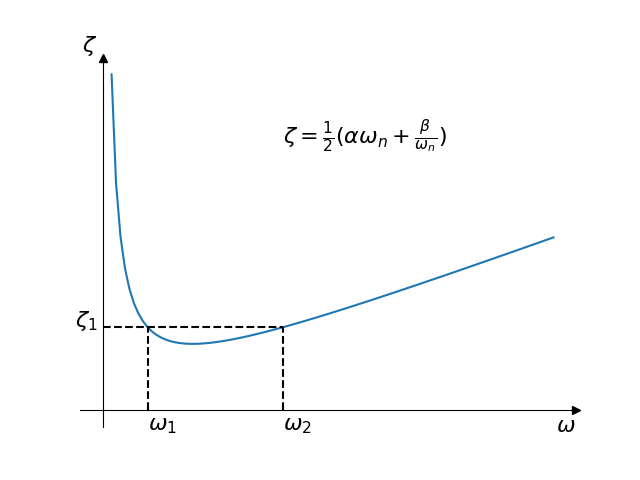
\includegraphics[width=0.90\textwidth]{img/general_rayleigh_damping.png}
    \caption{Schematic of full damping model}
    \label{fig:general-rayleigh-damping-png}
\end{figure}

In this case one needs two damping ratios and two natural frequencies to create
a pair of equations and solve for $ \alpha $ and $ \beta $. The model gives some
flexibility on where to place the natural frequencies, but in general, frequencies
too far away from the ones used in the computation will be amplified.

In the particular case of using equal damping ratios for the two frequencies,
it is important to note that the damping ratio \textbf{will not be constant inside the range}
defined by the sample points, but the inner frequencies will be attenuated. That is,
the inner frequencies will have a lower damping ratio.

\textbf{Computing the Rayleigh Damping Coefficients}

In the most common case, a transient response curve frim the system is obtained and
the damping ratio $ \zeta_1 $ is determined for the lowest natural frequency
$ \omega_1 $ by measuring the (logarithmic) attenuation of successive peaks.

\begin{figure}[ht]
    \centering
    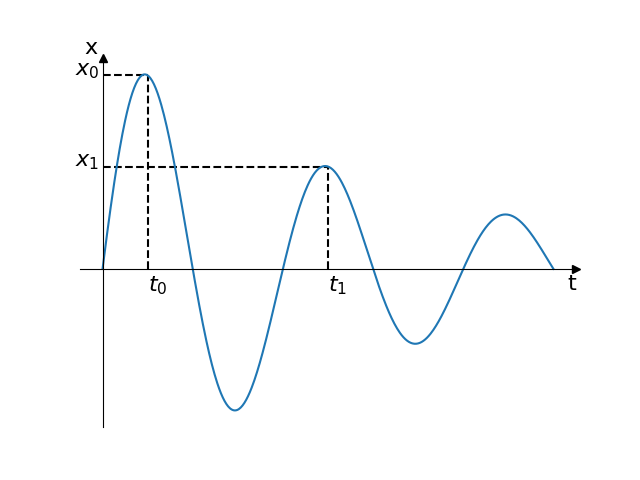
\includegraphics[width=0.90\textwidth]{img/Logarithmic_Decay_Damping_Ratio.png}
    \caption{Determination of the damping ration from the logarithmic decay}
    \label{fig:logarithmic-decay-damping-ratio-png}
\end{figure}

\begin{ematrix}
    \zeta &= \frac{\delta}{\sqrt{\delta^2 + (2 \pi)^2}}\\
    \delta &= \ln{\frac{x_0}{x_1}}\\
    f &= \frac{1}{T} = \frac{1}{t_1 - t_0}\\
    \omega &= 2 \pi f
\end{ematrix}

It is then most common to assume the case of damping proportional to the stiffness,
that is, $ \beta = 0 $, and the $ \alpha $ stiffness coefficient is computed from:

\begin{equation}
    \alpha = \frac{2 \zeta_1}{\omega_1} = \frac{\zeta+1}{\pi f_1}
\end{equation}

If the knowledge on the system indicates the case of damping decreasing with the
frequency, then one can assume the case of damping proportional to the inertia,
where $ \alpha = 0 $ and determine the mass coefficient $ \beta $:

\begin{equation}
    \beta = 2 \zeta_1 \omega_1 = 4 \pi \zeta_1 f_1
\end{equation}

If there is not such test data or knowledge of the system, or if one wishes to apply
an approximate damping ration over a range of frequencies, then we can use the
general case and build a system of two equations:

\begin{ematrix}
    \zeta_1 &= \frac{1}{2} \left( \alpha \omega_1 + \frac{\beta}{\omega_1} \right)\\
    \zeta_2 &= \frac{1}{2} \left( \alpha \omega_2 + \frac{\beta}{\omega_2} \right)
\end{ematrix}

Then solve for the unknown coefficients, keeping in mint the considerations given
above for the general case and the influence of the model on natural frequencies
inside and outside the range of interest. That is, perhaps one wants to achieve
a mean damping ratio over the range, then compensate the attenuation by modifying
the input damping rations, or by performing some least-squares approximation from
more than two frequency points.







\newpage
\section{Modal decomposition}

\subsection{Definition}

Let:

\begin{equation}
    \mathbf{M}\ddot{\mathbf{u}} + \mathbf{C}\dot{\mathbf{u}} +  \mathbf{K}\mathbf{u} = \mathbf{F}\left( t \right)
\end{equation}

be the \textbf{equation of motion}, then:\\
$ \mathbf{\Lambda} $ is a \textbf{spectral} matrix\\
$ \mathbf{\Psi} $ is a \textbf{mode shape} matrix,

such that:
\begin{equation}
    \mathbf{\Lambda} =
    \begin{bmatrix}
        \lambda_1^2 & \dots & 0\\
        \vdots & \ddots & \vdots \\
        0 & \dots & \lambda_n^2
    \end{bmatrix}
\end{equation}

where $ \lambda_n^2 $ is the n-th eigenvalue of the problem
$ (\mathbf{K}-\lambda^2\mathbf{M})\mathbf{X} = 0 $

and:
\begin{equation}
    \mathbf{\Psi} =
    \begin{bmatrix}
        \mathbf{\psi}_1 & \dots & \mathbf{\psi}_n
    \end{bmatrix}
\end{equation}

where $ \mathbf{\psi}_n = \{\psi_{n,1}, \dots, \psi_{n,m}\}^T $ is the eigenvector
of the n-th eigenvalue $ \lambda_n^2 $.

The \textbf{displacement} $ \mathbf{u} $ can be expressed as a linear combination
of eigenvectors such that:

\begin{ematrix}
    \mathbf{u}(t)
    &= \mathbf{\Psi} \mathbf{q}(t) \\
    &= \begin{bmatrix}
        \mathbf{\psi}_1 & \dots & \mathbf{\psi}_n
    \end{bmatrix} \mathbf{q}(t) \\
    &= \begin{bmatrix}
        \mathbf{\psi}_{1,1} & \dots & \mathbf{\psi}_{n,1} \\
        \vdots & \vdots & \vdots \\
        \mathbf{\psi}_{1,m} & \dots & \mathbf{\psi}_{n,m}
    \end{bmatrix}
    \begin{bmatrix}
        q_1(t) \\
        \vdots \\
        q_n(t)
    \end{bmatrix}
\end{ematrix}

where $ \mathbf{q}(t) $ is a vector of modal coefficients.

Then:

\begin{ematrix}
    \dot{\mathbf{u}}(t) &= \mathbf{\Psi} \dot{\mathbf{q}}(t) \\
    \ddot{\mathbf{u}}(t) &= \mathbf{\Psi} \ddot{\mathbf{q}}(t)
\end{ematrix}

First we substitute $ \mathbf{u} = \mathbf{\Psi}\mathbf{q} $ to the
\textbf{equation of motion}:

\begin{equation}
    \mathbf{M} \mathbf{\Psi} \ddot{q} +
    \mathbf{C} \mathbf{\Psi} \dot{q} +
    \mathbf{K}\mathbf{\Psi}\mathbf{q}
    = \mathbf{F}(t)
\end{equation}

By \textbf{premultiplying} with $ \mathbf{\Psi}^T $ we get:

\begin{equation}
    \mathbf{\Psi}^T \mathbf{M} \mathbf{\Psi} \ddot{\mathbf{q}} +
    \mathbf{\Psi}^T \mathbf{C} \mathbf{\Psi} \dot{\mathbf{q}} +
    \mathbf{\Psi}^T \mathbf{K} \mathbf{\Psi} \mathbf{q} =
    \mathbf{\Psi}\mathbf{F}(t) = \mathbf{Q}(t)
\end{equation}

where $ \mathbf{Q}(t) = \mathbf{\Psi} \mathbf{F}(t) $ is called a \textbf{modal load}.

\subsection{Orthonormalised Modal Base}

Then one can exploit the properties of \textbf{orthonormalised eigenvectors}, where:

\begin{equation}
    \mathbf{\psi}_r^T \mathbf{\psi}_s = 0 \Leftrightarrow r \neq s
\end{equation}

The \textbf{mass}, \textbf{damping} and \textbf{stiffness} matrices are therefore
reduced to:

\begin{ematrix}
    \mathbf{\Psi}^T \mathbf{M} \mathbf{\Psi}
    &= \begin{bmatrix}
        m_1 & \dots & 0 \\
        \vdots & \ddots & \vdots \\
        0 & \dots & m_n
    \end{bmatrix} \\
    \mathbf{\Psi}^T \mathbf{C} \mathbf{\Psi}
    &= \begin{bmatrix}
        c_1 & \dots & 0 \\
        \vdots & \ddots & \vdots \\
        0 & \dots & c_n
    \end{bmatrix} \\
    \mathbf{\Psi}^T \mathbf{K} \mathbf{\Psi}
    &= \begin{bmatrix}
        k_1 & \dots & 0 \\
        \vdots & \ddots & \vdots \\
        0 & \dots & k_n
    \end{bmatrix}
\end{ematrix}

where: \\
$ m_i $ is the \textbf{modal mass} of the i-th shape\\
$ c_i $ is the \textbf{modal damping} of the i-th shape\\
$ k_i $ is the \textbf{modal stiffness} of the i-th shape

\begin{bbox}[0.96]
    \textbf{Note}:

    When are the eigenvectors \textbf{orthonormalised} to \textbf{mass}, the above
    equations reduce to:

    \begin{ematrix}
        \mathbf{\Psi}^T \mathbf{M} \mathbf{\Psi}
        &= \begin{bmatrix}
            1.0 & \dots & 0 \\
            \vdots & \ddots & \vdots \\
            0 & \dots & 1.0
        \end{bmatrix} = \mathbf{I} \\
        \mathbf{\Psi}^T \mathbf{C} \mathbf{\Psi}
        &= \begin{bmatrix}
            c_1 & \dots & 0 \\
            \vdots & \ddots & \vdots \\
            0 & \dots & c_n
        \end{bmatrix} \\
        \mathbf{\Psi}^T \mathbf{K} \mathbf{\Psi}
        &= \begin{bmatrix}
            \lambda_1^2 & \dots & 0 \\
            \vdots & \ddots & \vdots \\
            0 & \dots & \lambda_n^2
        \end{bmatrix} = \mathbf{\Lambda}^2
    \end{ematrix}

    \textbf{Mass normalisation}:

    \begin{equation}
        \mathbf{\psi}_{i,mass} = \frac{\mathbf{\psi}_i}{\mathbf{\psi}_i^T \mathbf{m}_i \mathbf{\psi}_i}
    \end{equation}

    where:

    $ \mathbf{m}_i $ is the i-th row of the \textbf{mass} matrix $ \mathbf{M} $.

\end{bbox}


\subsection{MDOF to SDOF}

The MDOF \textbf{equation of motion} can be then rewritten as a set of \textbf{SDOF}
equations:

\begin{ematrix}
    \mathbf{\Psi}^T \mathbf{M} \mathbf{\Psi} \ddot{\mathbf{q}}(t) +
    \mathbf{\Psi}^T \mathbf{C} \mathbf{\Psi} \dot{\mathbf{q}}(t) +
    \mathbf{\Psi}^T \mathbf{K} \mathbf{\Psi} \mathbf{q}(t) &=
    \mathbf{\Psi}^T \mathbf{F}(t) \\
    \mathbf{M}_{\Psi} \ddot{\mathbf{q}}(t) +
    \mathbf{C}_{\Psi} \dot{\mathbf{q}}(t) +
    \mathbf{K}_{\Psi} \mathbf{q}(t) &= \mathbf{Q}(t)
\end{ematrix}

Written explicitely:

\begin{ematrix}
    \begin{bmatrix}
        m_1 & \dots & 0 \\
        \vdots & \ddots & \vdots \\
        0 & \dots & m_n
    \end{bmatrix}
    \begin{bmatrix}
        \ddot{q}_1(t) \\
        \vdots \\
        \ddot{q}_n(t)
    \end{bmatrix} &+ \\
    \begin{bmatrix}
        c_1 & \dots & 0 \\
        \vdots & \ddots & \vdots \\
        0 & \dots & c_n
    \end{bmatrix}
    \begin{bmatrix}
        \dot{q}_1(t) \\
        \vdots \\
        \dot{q}_n(t)
    \end{bmatrix} &+ \\
    \begin{bmatrix}
        k_1 & \dots & 0 \\
        \vdots & \ddots & \vdots \\
        0 & \dots & k_n
    \end{bmatrix}
    \begin{bmatrix}
        q_1(t) \\
        \vdots \\
        q_n(t)
    \end{bmatrix} &=
    \begin{bmatrix}
        Q_1(t) \\
        \vdots \\
        Q_n(t)
    \end{bmatrix}
\end{ematrix}

It is important to note that all modal matrices (mass, damping and stiffness) are
purely diagonal (with simple enough damping), so the \textbf{MDOF} problem reduces to a series
of \textbf{SDOF} problems:

\begin{ematrix}
    m_1 \ddot{q}_1(t) + c_1 \dot{q}_1(t) + k_1 q_1(t) &= Q_1(t) \\
    m_2 \ddot{q}_2(t) + c_2 \dot{q}_2(t) + k_2 q_2(t) &= Q_2(t) \\
    \vdots \\
    m_n \ddot{q}_n(t) + c_n \dot{q}_n(t) + k_n q_n(t) &= Q_n(t)
\end{ematrix}

which are solved separately and the results are \textbf{linearly} combined:

\begin{ematrix}
    \mathbf{u} = \sum_{i=1}^n \mathbf{\psi}_i q_i \\
    \mathbf{\dot{u}} = \sum_{i=1}^n \mathbf{\psi}_i \dot{q}_i \\
    \mathbf{\ddot{u}} = \sum_{i=1}^n \mathbf{\psi}_i \ddot{q}_i
\end{ematrix}

\begin{bbox}[0.96]
    \textbf{Note:} Above equation can be also written as:

    \begin{ematrix}
        \mathbf{u} = \sum_{i=1}^n \mathbf{\psi}_i q_{u,i} \\
        \mathbf{v} = \sum_{i=1}^n \mathbf{\psi}_i q_{v,i} \\
        \mathbf{a} = \sum_{i=1}^n \mathbf{\psi}_i q_{a,i}
    \end{ematrix}

    where:\\
    $ \mathbf{u} $ is displacement \\
    $ \mathbf{v} $ is velocity \\
    $ \mathbf{a} $ is acceleration

    and\\
    $ \mathbf{q}_{u} $ is modal displacement \\
    $ \mathbf{q}_v $ is modal velocity \\
    $ \mathbf{q}_a $ is modal acceleration

\end{bbox}


\subsection{Initial Conditions}

To get the initial modal conditions, one simply:

\begin{ematrix}
    \mathbf{q}_0 &= \mathbf{\Psi}^{-1} \mathbf{u}_0 \\
    \mathbf{\dot{q}}_0 &= \mathbf{\Psi}^{-1} \mathbf{\dot{u}}_0 \\
    \mathbf{\ddot{q}}_0 &= \mathbf{\Psi}^{-1} \mathbf{\ddot{u}}_0
\end{ematrix}

where:\\
$ \mathbf{\Psi}^{-1} $ is an inverse of eigenshape matrix $ \Leftrightarrow $ all eigenvalues
and eigenshapes are used.

\begin{bbox}[0.96]
    \textbf{Note}: This is not usually so. Normally one would use
    \textbf{reduced modal base}, where only the first \textbf{n} eigenmodes are used. Then
    $ \mathbf{\Psi}^{-1} $ is written as $ \mathbf{\Psi}^{+} $ and called the
    \textbf{pseudoinverse of mode shape matrix} defined (at least in \textbf{numpy}
    - \textit{numpy.linal.pinv()}) as:\\

    \smallskip
    The pseudo-inverse of a matrix $ \mathbf{A} $, denoted $ \mathbf{A}^{+} $,
    is defined as: “the matrix that ‘solves’ [the least-squares problem]
    $ \mathbf{A} \mathbf{x} = \mathbf{b} $ ,” i.e., if $ \overline{\mathbf{x}} $
    is said solution, then $ \mathbf{A}^{+} $ is that matrix such that
    $ \overline{\mathbf{x}} = \mathbf{A}^{+} \mathbf{b} $.\\

    \smallskip
    It can be shown that if $ \mathbf{Q}_1 \mathbf{\Sigma} \mathbf{Q}_2^T = \mathbf{A} $
    is the singular value decomposition of $ \mathbf{A} $, then
    $ \mathbf{A}^{+} = \mathbf{Q}_2 \mathbf{\Sigma}^{+} \mathbf{Q}_1^T $, where $ \mathbf{Q}_{1,2} $
    are orthogonal matrices, $ \mathbf{\Sigma} $  is a diagonal matrix consisting of
    $ \mathbf{A} $’s so-called singular values, (followed, typically, by zeros),
    and then $ \mathbf{\Sigma}^{+} $ is simply the diagonal matrix consisting
    of the reciprocals of $ \mathbf{A} $’s singular values (again, followed
    by zeros).
\end{bbox}




\chapter{Iterative Methods}

\section{second order ODE's}

Most of FEM problems are \textbf{second order Ordinary Differential Equations}, e.g:

\begin{ematrix}
    m \frac{u''(t)}{d^2 t} + c \frac{u'(t)}{dt} + k u(t) &= 0\\
    m \ddot{u} + c \dot{u} + k u &= 0\\
    m a + c v + ku &= 0
\end{ematrix}

while the iterative methods are for \textbf{first order ODE's} only.
A \textbf{substitution} technique is therefore used to transform the
\textbf{second order ODE's} to a set of \textbf{first order ODE's} and these are
then solved sequentialy.

First we begin with a \textbf{second order ODE} in the form of:

\begin{equation}
    a \frac{y''(x)}{d^2 x} + b \frac{y'(x)}{dx} + c y = d, \quad with \quad y(0) = y_0 \quad and \quad
    \frac{y'(0)}{dx} = y_1
\end{equation}

By stating:

\begin{equation}
    \frac{dy}{dx} = z
\end{equation}

and substituting back:

\begin{equation}
    a \frac{dz}{dx} + b z + c y = d
\end{equation}

now we can write the following set of equations:

\begin{ematrix}
    \begin{aligned}
        z &= \frac{dy}{dx}\\
        \frac{dz}{dx} &= \frac{d - c y - b z}{a}
    \end{aligned} &
    \quad \left\{
    \begin{aligned}
        y(0) &= y_0\\
        z(0) &= y_1
    \end{aligned} \right.
\end{ematrix}



\section{Explicit}

\subsection{Euler's method}
The \textbf{Euler's Method} is an iterative method to solve ODEs. This method's
huge plus is it is fast. The minus is it gradually diverges from the ideal solution.

The \textbf{Euler's Method} uses the following formula:

\begin{equation}
    y(t + h) = y(t) + h f(x,y)
\end{equation}

to construct the tangent at point $ x $ and obtain the value of $ y(x + h) $,
whose slope is:

\begin{equation}
    f(x,y) \quad or \quad \frac{dy}{dx}
\end{equation}

\begin{figure}[ht]
    \centering
    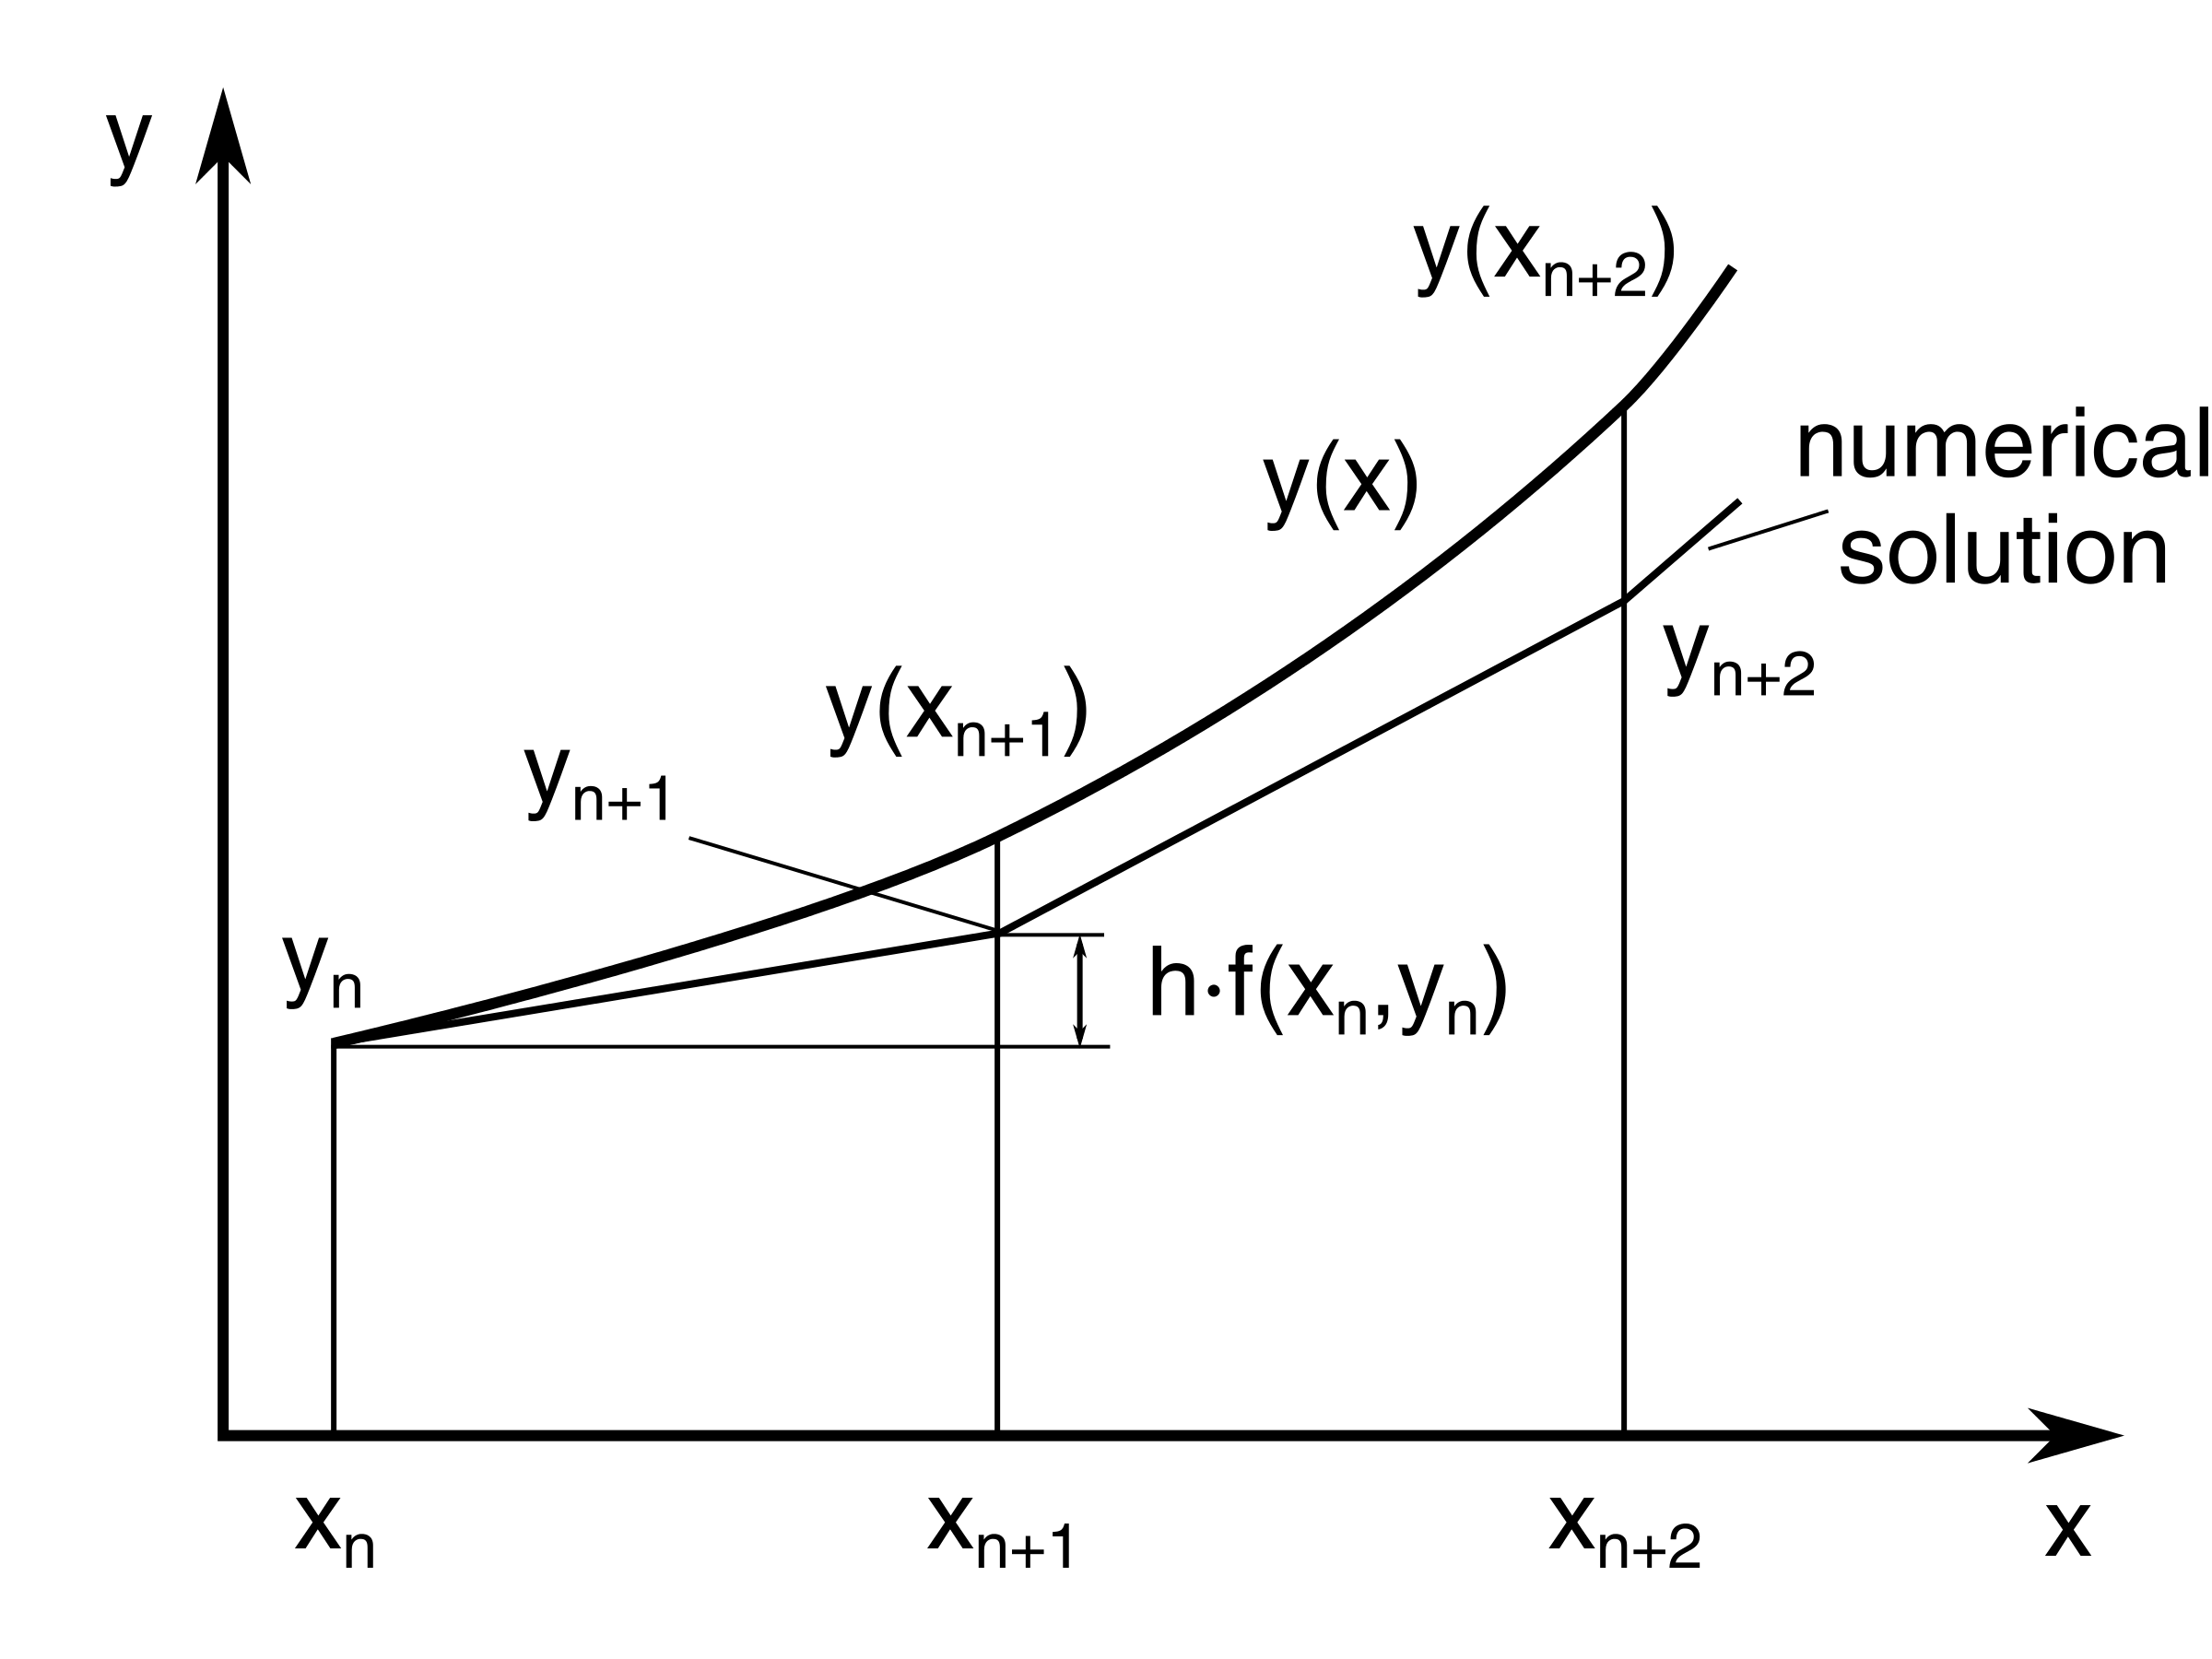
\includegraphics[width=0.90\textwidth]{img/Euler.png}
    \caption{Euler's method schematic}
    \label{fig:euler-png}
\end{figure}

In Euler's method, you can approximate the curve of the solution byt the tangent
in each interval (that is, by a sequence of shor line segments), at steps of $ h $.

\textit{In general}, if you use small step size, the accuracy of the approximation
increases.

\textbf{General Formula}

\begin{equation}
    y_{i+1} = y_i + h f(x_i,y_i)
\end{equation}

where:\\
$ y_{i+1} $ is the next estimated solution value,\\
$ y_i $ is the current value,\\
$ h $ is the interval between steps and\\
$ f(x_i,y_i) $ is the value of the derivative at the current $ (x_i,y_i) $ point.

\textbf{Pseudocode:}

\begin{itemize}
    \item define: $ f(x,y) $

    \item input: $ x_0 $, $ y_0 $

    \item input: $ h $, $ n $

    \item for $ j $ from $ 0 $ to $ (n-1) $ do
        \begin{itemize}
            \item $ y_{j+1} = y_j + hf(x_j, y_j) $
            \item $ x_{j+1} = x_j + h $
            \item Print $ x_{j+1} $ and $= y_{j+1} $
        \end{itemize}
    \item End.
\end{itemize}


\begin{bbox}[0.96]
\textbf{Note:}

If thinking about a problem in time domain:

\begin{itemize}
    \item define: $ f(t,x) $

    \item input: $ t_0 $, $ x_0 $

    \item input: $ dt $, $ n $

    \item for $ j $ from $ 0 $ to $ (n-1) $ do
        \begin{itemize}
            \item $ x_{j+1} = x_j + dt f(t_j, x_j) $
            \item $ t_{j+1} = t_j + dt $
            \item Print $ t_{j+1} $ and $= x_{j+1} $
        \end{itemize}
    \item end.
\end{itemize}

\end{bbox}


\newpage
\textbf{Python Code for vibration problem:}

\begin{python}
#!/usr/bin/python3
import numpy as np
import matplotlib.pyplot as plt


def iterate(h, y0, func, rhs):
    num_of_odes = y0.shape[0]
    y1 = np.zeros(num_of_odes, dtype = float)
    for i in range(num_of_odes-1):
        y1[i] = y0[i] + y0[i+1] * h
    y1[-1] = func(y1, rhs)
    return y1


def euler(t, y, func, rhs):
    N = t.shape[0]
    for j in range(N-1):
        dt = t[j+1] - t[j]
        y[j+1,:] = iterate(dt, y[j,:], func, rhs[j])
        # print(y[j+1,:])
    return y


def euler_vibration():
    m = 0.55  # tonnes
    c = 3.    # Ns/mm
    k = 1000. # N/mm

    freq = np.sqrt(k / m) / (2 * np.pi)

    # equation to solve
    # m * a + c * v + k * u = f
    # a = (f - c * v - k * u) / m
    acceleration = lambda u, f: (f - c * u[1] - k * u[0]) / m

    T = 2.0     # seconds
    dt = 0.0001 # timestep s
    u_0 = 0.    # mm of initial displacement
    v_0 = 0.    # mm/s of initial velocity

    # times at which to solve
    t = np.linspace(0, T, int(T/dt) + 1)

    # force vector
    F = 5000. # N of max impulse
    t0 = 0.1  # impulse start time
    t1 = 0.2  # impuls end time
    f = np.zeros(t.shape[0], dtype=float)
    # create a half sine impulse of force
    for i in range(t.shape[0]):
        if t[i] >= t0 and t[i] <= t1:
            f[i] = F * np.sin((t[i] - t0) / (t1 - t0) * np.pi)
        else:
            f[i] = 0.

    uva = np.zeros((t.shape[0],3), dtype=float)
    uva[0,0] = u_0
    uva[0,1] = v_0

    uva = euler(t, uva, acceleration, f)

    fig, axf = plt.subplots()
    fig.subplots_adjust(right=0.60)

    p1, = axf.plot(t, f, label='force', color='violet')
    axu = axf.twinx()
    p2, = axu.plot(t, uva[:,0], label='displacement', color='red')
    axv = axf.twinx()
    axv.spines.right.set_position(('axes', 1.20))
    p3, = axv.plot(t, uva[:,1], label='velocity', color='blue')
    axa = axf.twinx()
    axa.spines.right.set_position(('axes', 1.40))
    p4, = axa.plot(t, uva[:,2], label='acceleration', color='green')

    axf.set_xlabel('Time [s]')
    axf.set_ylabel('Force [N]')
    axu.set_ylabel('Displacement [mm]')
    axv.set_ylabel('Velocity [mm/s]')
    axa.set_ylabel('Acceleration [mm/s2]')

    axf.legend(handles=[p1, p2, p3, p4])

    plt.show()

if __name__ == '__main__':
    euler_vibration()

\end{python}

Which results to:
\begin{figure}[ht]
    \centering
    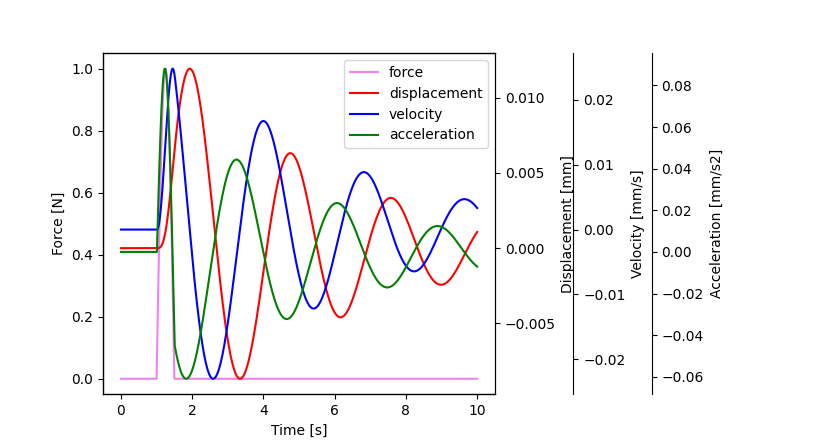
\includegraphics[width=0.90\textwidth]{img/euler_example.png}
    \caption{Euler's implementation for vibration problem example}
    \label{fig:euler-example-png}
\end{figure}


The \textbf{iterate()} function:
\begin{python}
def iterate(h, y0, func, rhs):
    num_of_odes = y0.shape[0]
    y1 = np.zeros(num_of_odes, dtype = float)
    for i in range(num_of_odes-1):
        y1[i] = y0[i] + y0[i+1] * h
    y1[-1] = func(y1, rhs)
    return y1

\end{python}

is written for general case of a set of ODEs. When considering the problem
of vibration (set of 2 ODEs):
\begin{python}
def iterate(h, u0, v0, a0, f, m , c, k):
    u1 = u0 + h * v0
    v1 = v0 + h * a0
    # m * a + c * v + k * u = f
    a1 = (f - c * v1 - k * u1) / m
    return np.array([u1, v1, a1], dtype=float)
\end{python}

which is the iteration of a set of \textbf{first order ODEs}:
\begin{ematrix}
    v &= \dot{u}\\
    \dot{v} &= \frac{f - c * v - k * u}{m}
\end{ematrix}

\newpage
\subsection{Runge-Kutta 4th order method}

\textbf{Runge-Kutta 4th order method} is another explicit method for solving
\textbf{first order ODEs}. The basic equation is:

\begin{equation}
    \frac{dy}{dx} = f(x,y) \quad , y(0) = y_0
\end{equation}

The formula for the next value $ y_{i+1} $ after a step size equal to $h $ is given by:

\begin{ematrix}
    k_1 &= h f(x_i, y_i)\\
    k_2 &= h f(x_i + \frac{h}{2}, y_i + \frac{k_1}{2})\\
    k_3 &= h f(x_i + \frac{h}{2}, y_i + \frac{k_2}{2})\\
    k_4 &= h f(x_i + h, y_i + k_3)\\
    y_{i+1} &= y_i + \frac{k_1}{6} + \frac{k_2}{3} + \frac{k_3}{3} + \frac{k_4}{6} + O(h^5)
\end{ematrix}

The formula basically computes next value $ y_{i+1} $ using current $ y_i $ plus
\textbf{weighted average of four increments}:

\begin{itemize}
    \item $ k_1 $ is the increment based on the slope at the beginning of the
    interval, using $ y $

    \item $ k_2 $ is the increment based on the slope at the midpoint of the interval,
        using $ y + h k_1 / 2 $

    \item $ k_3 $ is the increment based on the slope at the midpoint,
        using $ y + h k_2 / 2 $

    \item $ k_4 $ is the increment based on the slope at the end of the interval,
        using $ y + h k_3 / 2 $

\end{itemize}

The method is a fourth order method, meaning that the local truncation error is
on the order of $ O(h^5) $, while the total accumulated error is of order $ O(h^4) $.

\begin{figure}[ht]
    \centering
    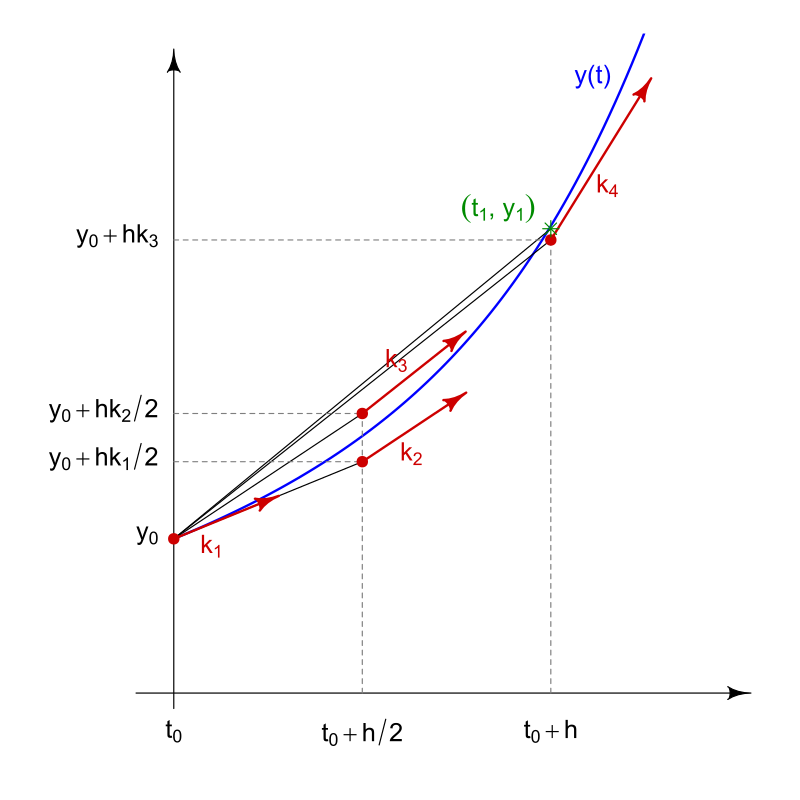
\includegraphics[width=0.80\textwidth]{img/Runge-Kutta_slopes.png}
    \caption{4th Order Runge-Kutta's method schematic}
    \label{fig:rk4-schema-png}
\end{figure}

\newpage
\begin{bbox}[0.96]
\textbf{Note:}

The formula for the next value $ y_{i+1} $ can be also written as:

\begin{ematrix}
    k_1 &= y_i\\
    k_2 &= y_i + \frac{h}{2} \frac{d k_1}{dx}\\
    k_3 &= y_i + \frac{h}{2} \frac{d k_2}{dx}\\
    k_4 &= y_i + h \frac{k_3}{dx}\\
    y_{i+1} &= y_i + \frac{h}{6} (\frac{d k_1}{dx} + 2 \frac{d k_2}{dx}
                              + 2 \frac{d k_3}{dx} + \frac{d k_4}{dx}) + O(h^5)
\end{ematrix}
\end{bbox}

\begin{bbox}[0.96]
This notation is more convenient to use when solving sets of ODEs for vibration
problem, because it translates to:

\begin{ematrix}
    u_1 &= u_0\\
    v_1 &= v_0\\
    a_1 &= (f - c v_0 - k u_0) / m\\
    u_2 &= u_0 + \frac{h}{2} v_1\\
    v_2 &= v_0 + \frac{h}{2} a_1\\
    a_2 &= (f - c v_1 - k u_1) / m\\
    u_3 &= u_0 + \frac{h}{2} v_2\\
    v_3 &= v_0 + \frac{h}{2} a_2\\
    a_3 &= (f - c v_2 - k u_2) / m\\
    u_4 &= u_0 + h v_3\\
    v_4 &= v_0 + h a_3\\
    a_4 &= (f - c v_3 - k u_3) / m\\
    u_{i+1} &= u_0 + \frac{h}{6} \left( v_1 + 2 v_2 + 2 v_3 + v_4 \right) \\
    v_{i+1} &= v_0 + \frac{h}{6} \left( a_1 + 2 a_2 + 2 a_3 + a_4 \right) \\
    a_{i+1} &= (f - c v_{i+1} - k u_{i+1}) / m\\
\end{ematrix}

where each of the \textbf{ODEs} are solved sequentially from the values
already known.

\end{bbox}

\newpage
\textbf{Python implementation for vibration problem:}

\begin{python}
#!/usr/bin/python3
import numpy as np
import matplotlib.pyplot as plt


def iterate(h, y0, y, func, rhs):
    num_of_odes = y0.shape[0]
    y1 = np.zeros(num_of_odes, dtype = float)
    for i in range(num_of_odes-1):
        y1[i] = y0[i] + y[i+1] * h
    y1[-1] = func(y1, rhs)
    return y1


def runge_kutta_4(t, y, func, rhs):
    N = t.shape[0]
    for j in range(N-1):
        dt = t[j+1] - t[j]
        y1 = iterate(0., y[j,:], y[j,:], func, rhs[j])
        y2 = iterate(dt/2, y[j,:], y1, func, 0.5 * (rhs[j+1] + rhs[j]))
        y3 = iterate(dt/2, y[j,:], y2, func, 0.5 * (rhs[j+1] + rhs[j]))
        y4 = iterate(dt, y[j,:], y3, func, rhs[j+1])

        # next step solution
        for i in range(y.shape[1]-1):
            y[j+1,i] = y[j,i] + dt/6 * (y1[i+1] + 2 * y2[i+1] + 2 * y3[i+1] + y4[i+1])
        y[j+1,-1] = func(y[j+1,:], rhs[j+1])
    return y


def rk4_vibration():
    m = 10.   # tonnes
    c = 5.    # Ns/mm
    k = 50.   # N/mm

    freq = np.sqrt(k / m) / (2 * np.pi)
    print(f'f = {freq}')

    # equation to solve
    # m * a + c * v + k * u = f
    # a = (f - c * v - k * u) / m
    acceleration = lambda u, f: (f - c * u[1] - k * u[0]) / m

    T = 10.     # seconds
    dt = 0.01   # timestep s
    u_0 = 0.    # mm of initial displacement
    v_0 = 0.    # mm/s of initial velocity

    # times at which to solve
    t = np.linspace(0, T, int(T/dt) + 1)

    # force vector
    F = 1.    # N of max impulse
    t0 = 1.   # impulse start time
    t1 = 1.5  # impuls end time
    f = np.zeros(t.shape[0], dtype=float)
    # create a half sine impulse of force
    for i in range(t.shape[0]):
        if t[i] >= t0 and t[i] <= t1:
            f[i] = F * np.sin((t[i] - t0) / (t1 - t0) * np.pi)
        else:
            f[i] = 0.

    uva = np.zeros((t.shape[0],3), dtype=float)
    uva[0,0] = u_0
    uva[0,1] = v_0

    uva = runge_kutta_4(t, uva, acceleration, f)

    fig, axf = plt.subplots()
    fig.subplots_adjust(right=0.60)

    p1, = axf.plot(t, f, label='force', color='violet')
    axu = axf.twinx()
    p2, = axu.plot(t, uva[:,0], label='displacement', color='red')
    axv = axf.twinx()
    axv.spines.right.set_position(('axes', 1.20))
    p3, = axv.plot(t, uva[:,1], label='velocity', color='blue')
    axa = axf.twinx()
    axa.spines.right.set_position(('axes', 1.40))
    p4, = axa.plot(t, uva[:,2], label='acceleration', color='green')

    axf.set_xlabel('Time [s]')
    axf.set_ylabel('Force [N]')
    axu.set_ylabel('Displacement [mm]')
    axv.set_ylabel('Velocity [mm/s]')
    axa.set_ylabel('Acceleration [mm/s2]')

    axf.legend(handles=[p1, p2, p3, p4])

    plt.show()

if __name__ == '__main__':
    rk4_vibration()

\end{python}

Which results to:
\begin{figure}[ht]
    \centering
    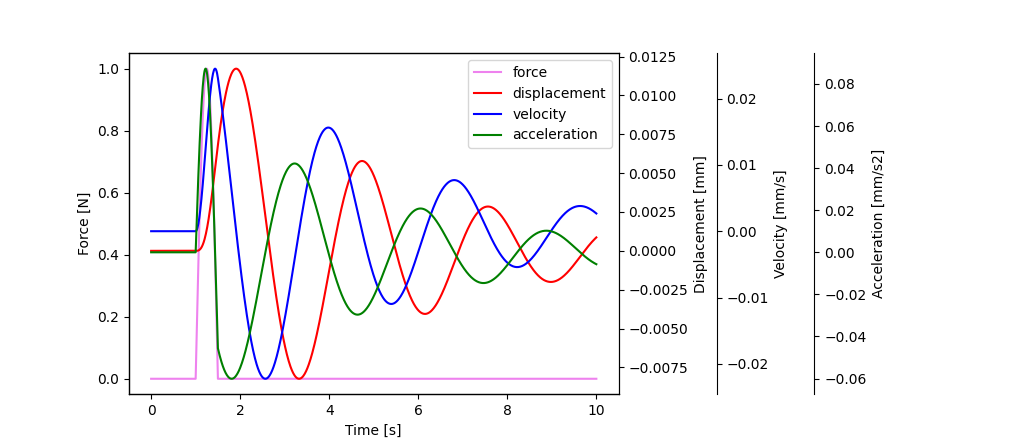
\includegraphics[width=0.90\textwidth]{img/rk4_example.png}
    \caption{4th order Runge-Kutta's implementation for vibration problem example}
    \label{fig:rk4-example-png}
\end{figure}



\end{document}

